\documentclass[12pt]{article}
\usepackage[top = 2.5cm, bottom = 2.5cm, left = 2.5cm, right = 2.5cm]{geometry}
\usepackage{listings}
\usepackage{color} % red, green, blue, yellow, cyan, magenta, black, white
\usepackage{amsmath}
\usepackage{amssymb}
\usepackage{bm}
\usepackage{enumerate}
\usepackage{graphicx}
\usepackage{float}
\usepackage{booktabs}
\usepackage{makecell}
\usepackage[hidelinks]{hyperref}
\usepackage{multicol}
\usepackage{multirow}
\usepackage{cite}
\usepackage{bbding} % checkmarks
\usepackage{fancyhdr} % change the position of page number
\usepackage[flushleft]{threeparttable} % footnote in tables
\usepackage{lipsum}
\usepackage{caption}
\captionsetup{format = hang}
\usepackage{color, colortbl} % coloring rows or columns in tables
\definecolor{Gray}{gray}{.9} % coloring rows or columns in tables
\definecolor{darkgreen}{RGB}{0,100,0}
\definecolor{darkred}{RGB}{100,0,0}
\newcommand{\horrule}[1]{\rule{\linewidth}{#1}}
\fancyhf{} % clear all header and footers
\renewcommand{\headrulewidth}{0pt} % remove the header rule
\rfoot{\thepage} % puts the page number on the right side
\pagestyle{fancy}
\title{Spider plots}
\date{\today}
\author{Henrique Laureano\\
        \texttt{https://henriquelaureano.github.io/}}

\begin{document}

\maketitle
\thispagestyle{empty}

\vfill
\noindent \horrule{.5pt} \vspace{-.95cm} \tableofcontents \noindent \horrule{.5pt}

\section*{Coefficients}
\addcontentsline{toc}{section}{Coefficients}

Based on the fitted model parameters, the predicted values were obtained
for four different profiles focused on four different features:
pesticides reduction, unbreakable contract, penalization, and contract
length. The variables that compose each profile can be accessed on the
right table of \autoref{fig:spider}.

\begin{figure}[H]
 \centering
 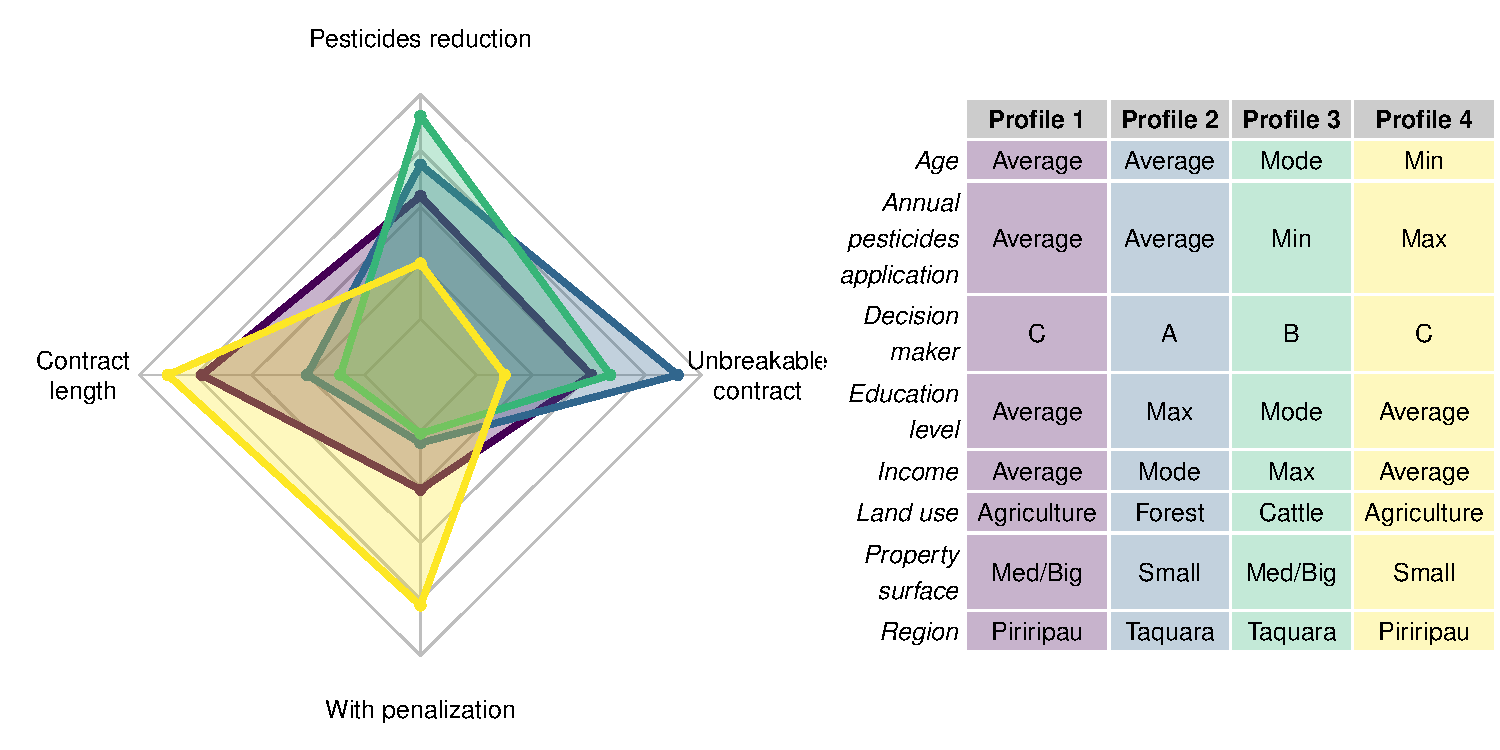
\includegraphics[width=\textwidth]{figures/spider.pdf}\\
 \caption{Spider chart for four variables based on the four most
          frequent profiles and their model coefficients}
 \label{fig:spider}
\end{figure}

With \autoref{fig:spider} and \autoref{fig:spiders}, we see a clear
difference between the profiles, showing that even with each profile
being built by a considerable number of features, each of those features
is relevant - given the considerable differences obtained in terms of
predicted values from one profile to another. Each profile is
highlighted in one direction/variable, which also shows that based on
those four profiles we are able to virtually reach all possible
spectrums since we basically reach all vertices of the spider chart. In
\autoref{fig:spider} we see all of them together, and in
\autoref{fig:spiders}, side=by-side. In three of the four features,
profile 4 presents the most extreme values.

\begin{figure}[H]
 \centering
 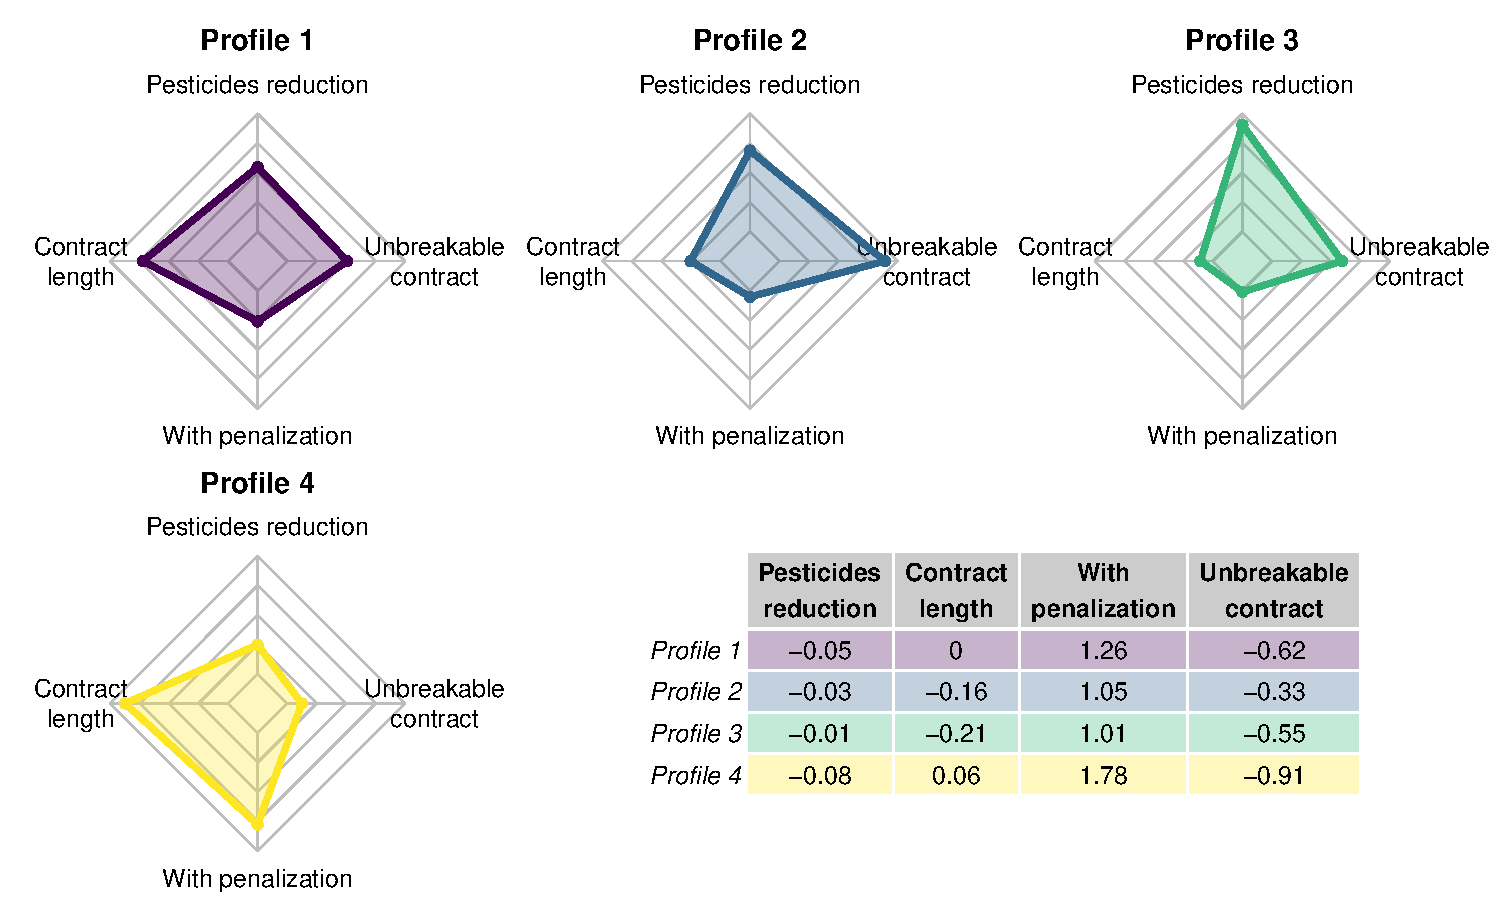
\includegraphics[width=\textwidth]{figures/spiders.pdf}\\
 \caption{Spider charts for four variables based on the four most
          frequent profiles and their model coefficients}
 \label{fig:spiders}
\end{figure}

\section*{WTA profit}
\addcontentsline{toc}{section}{WTA profit}

In \autoref{fig:spider_wta} and \autoref{fig:spiders_wta}, we now look
at the WTA profits per feature and profile. We can still see clear
differences between the profiles, with each one highlighting a different
feature. Again, the most extremes values are obtained with profile 4.

\begin{figure}[H]
 \centering
 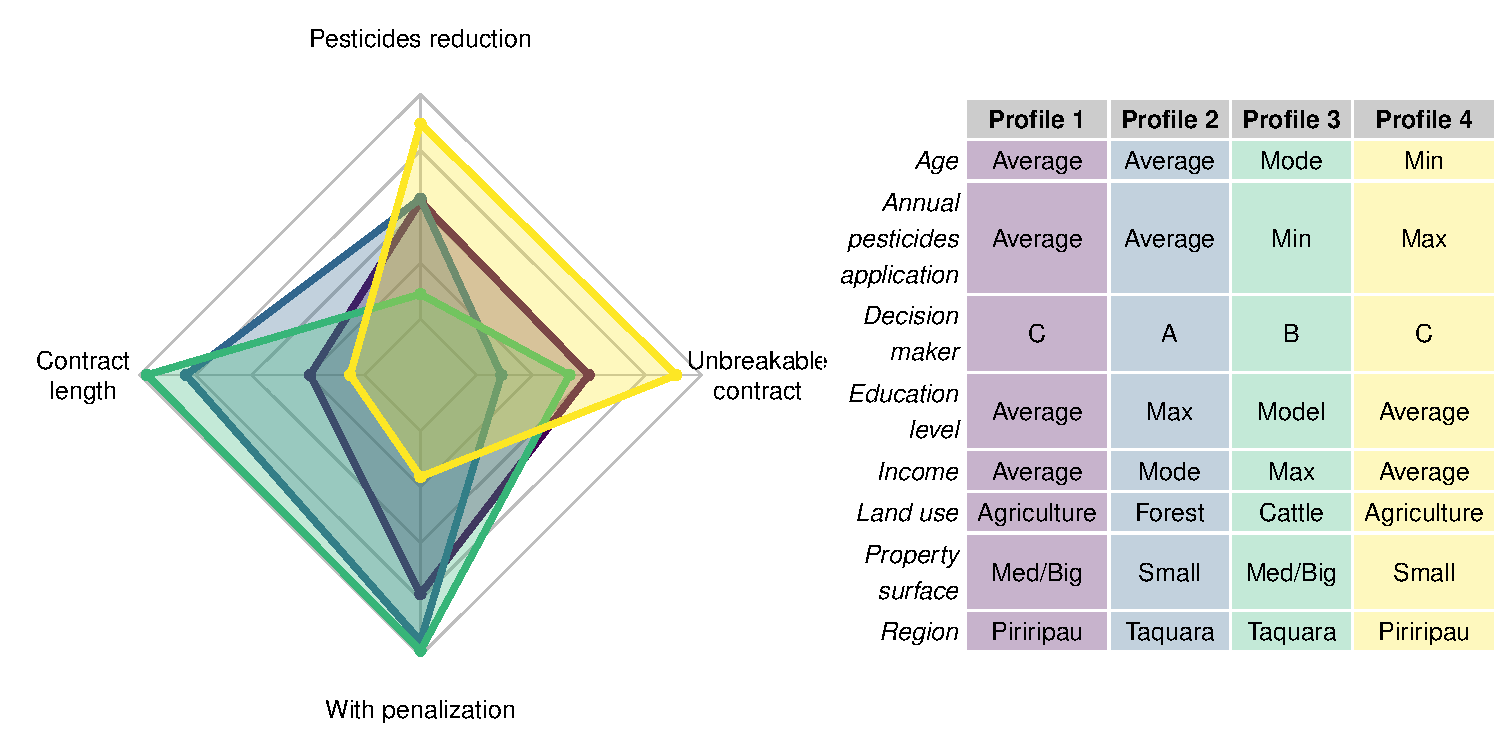
\includegraphics[width=\textwidth]{figures/spider_wta.pdf}\\
 \caption{Spider chart for four variables based on the four most
          frequent profiles and their WTA profits}
 \label{fig:spider_wta}
\end{figure}

\begin{figure}[H]
 \centering
 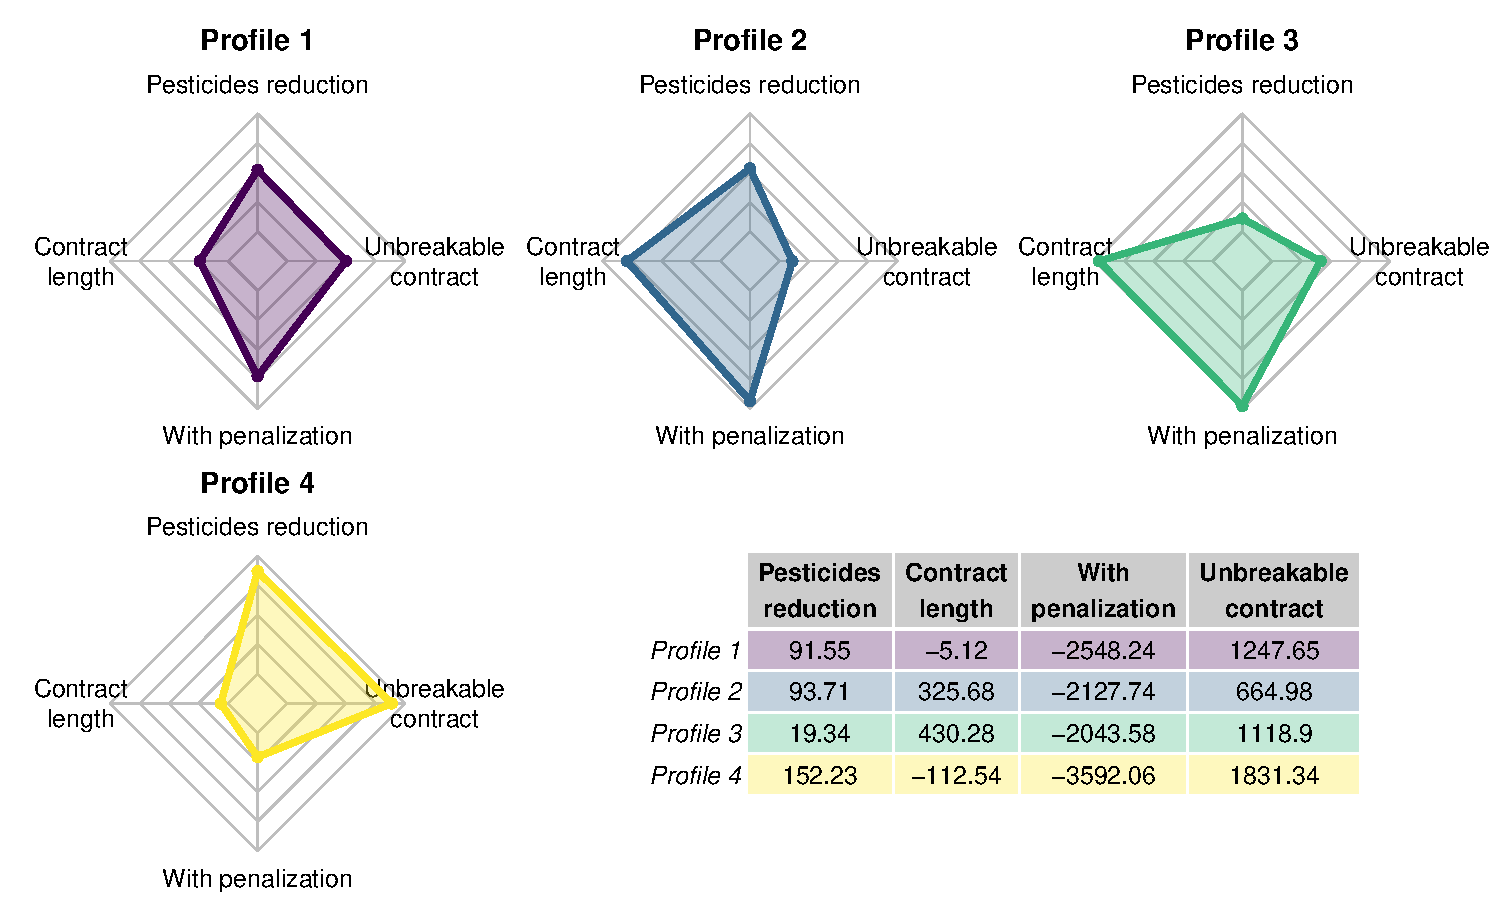
\includegraphics[width=\textwidth]{figures/spiders_wta.pdf}\\
 \caption{Spider charts for four variables based on the four most
          frequent profiles and their WTA profits}
 \label{fig:spiders_wta}
\end{figure}

\section*{Scenarios}
\addcontentsline{toc}{section}{Scenarios}

In \autoref{fig:scenarios}, we have the total amount to be payed in each
of the four profiles in six different scenarios. We see that the
profiles behaviors are not the same, varying depending on the scenario
and turning out to be very difficult to state any clear pattern besides
the fact that scenario 11 present the biggest general amounts, and that
scenario 9 presents the general smallest.

\begin{figure}[H]
 \centering
 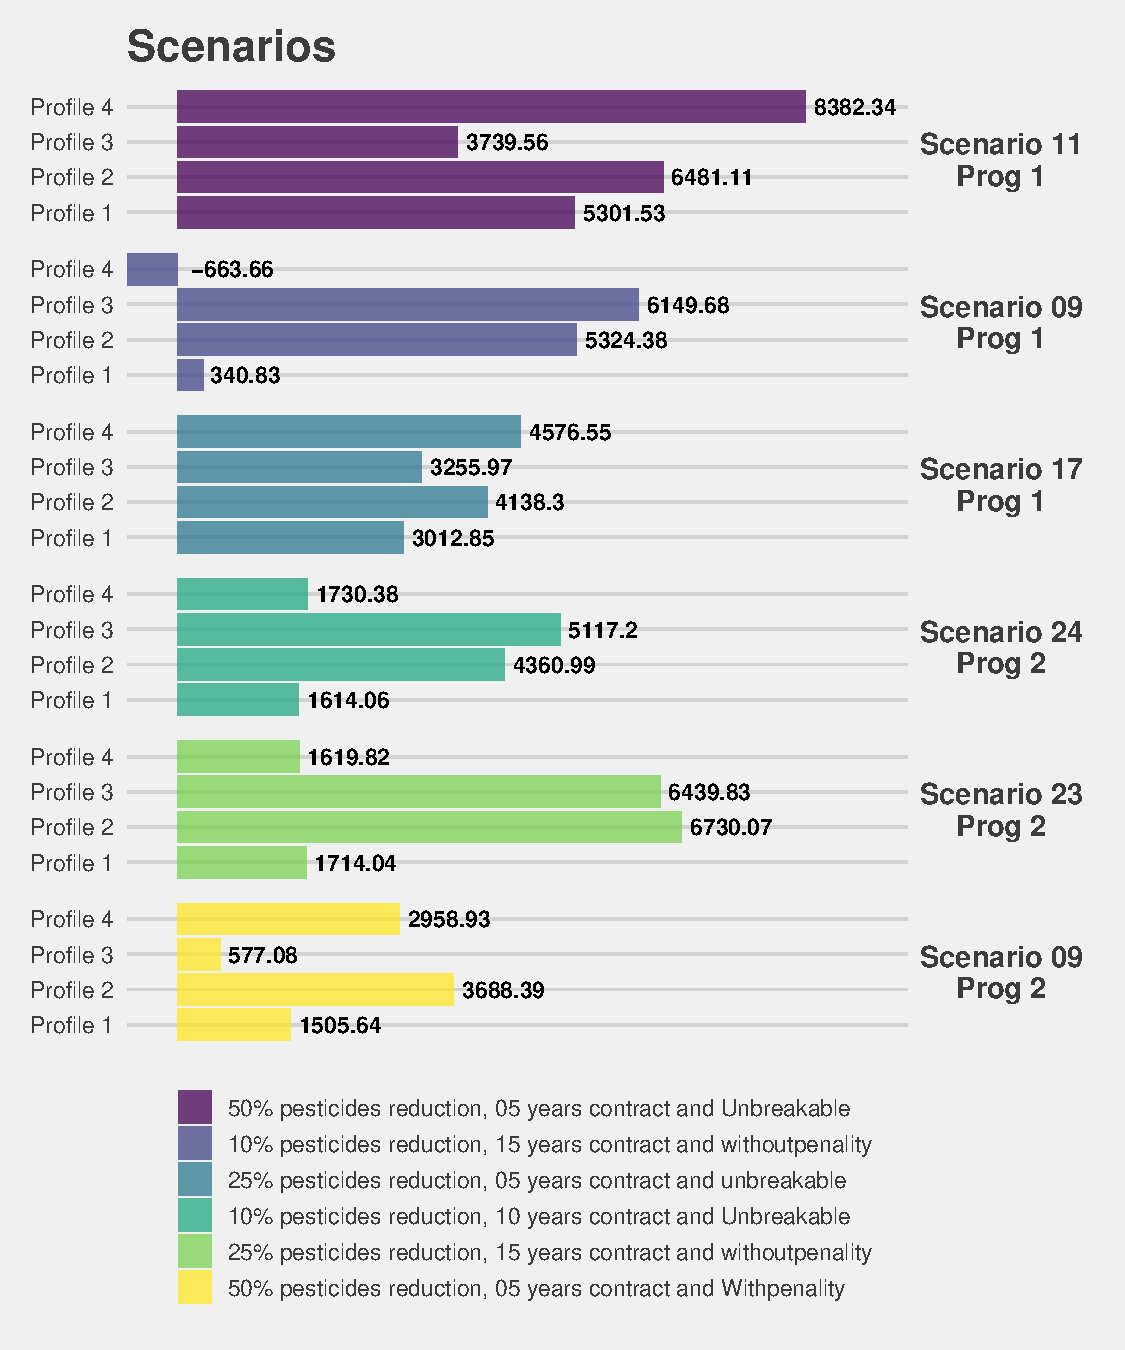
\includegraphics[width=0.875\textwidth]{figures/scenarios.pdf}\\
 \caption{Total amount to be payed for six different scenarios and four
          profiles}
 \label{fig:scenarios}
\end{figure}

\section*{Model formula}
\addcontentsline{toc}{section}{Model formula}

\begin{align*}
 \texttt{Profile 1}_{~\texttt{Pesticides reduction}}
 &= -0.04568\\
 &+ 0.0004559 \times \texttt{\textit{Average} Age}\\
 &- 0.000001664 \times \texttt{\textit{Average} Annual pesticides application}\\
 %% &+ \beta \times \texttt{Decision maker \textit{C}}\\
 &- 0.0003879 \times \texttt{\textit{Average} Education level}\\
 &- 0.00239 \times \texttt{\textit{Average} Income}\\
 %% &+ \beta \times \texttt{\textit{Agriculture} Land use}\\
 %% &+ \beta \times \texttt{\textit{Medium/Big} Property surface}\\
 %% &+ \beta \times \texttt{\textit{Piriripau} Region}
 \\
 \texttt{Profile 1}_{~\texttt{Contract length}}
 &= -0.1038\\
 &- 0.0002863 \times \texttt{\textit{Average} Age}\\
 &+ 0.00007659 \times \texttt{\textit{Average} Annual pesticides application}\\
 %% &+ \beta \times \texttt{Decision maker \textit{C}}\\
 &- 0.003189 \times \texttt{\textit{Average} Education level}\\
 &+ 0.0131 \times \texttt{\textit{Average} Income}\\
 %% &+ \beta \times \texttt{\textit{Agriculture} Land use}\\
 %% &+ \beta \times \texttt{\textit{Medium/Big} Property surface}\\
 %% &+ \beta \times \texttt{\textit{Piriripau} Region}
 \\
 \texttt{Profile 1}_{~\texttt{With penalization}}
 &= 2.2660\\
 &- 0.01639 \times \texttt{\textit{Average} Age}\\
 %% &+ \beta \times \texttt{Decision maker \textit{C}}\\
 &+ 0.07299 \times \texttt{\textit{Average} Education level}\\
 &- 0.03419 \times \texttt{\textit{Average} Income}\\
 \\
 \texttt{Profile 1}_{~\texttt{Unbreakable contract}}
 &= -1.2640\\
 &+ 0.009166 \times \texttt{\textit{Average} Age}\\
 %% &+ \beta \times \texttt{Decision maker \textit{C}}\\
 &+ 0.1232 \times \texttt{\textit{Average} Education level}\\
 &- 0.03151 \times \texttt{\textit{Average} Income}
\end{align*}

\end{document}
